\chapter{Q-Function Methods}
Recall the algorithms that we discussed in last chapter: Alg. \ref{alg:fittedQ} and Alg. \ref{alg:onlineQiter}, where we devised a fitted Q-learning algorithm and a fully online version of it. We have also shown that Q-learning is fully off-policy, meaning that we do not care about the trajectory we are taking, we only care about the current transition and the next state we land in. So what is the problem with the above Q-learning algorithms? To see this, let us carefully look at step 4 of Alg. \ref{alg:onlineQiter}. The gradient step that we are taking is equivalently written as:
$$\phi\leftarrow \phi - \alpha\frac{dQ_\phi}{d\phi}(s_i,a_i)\left(Q_\phi(s_i,a_i) - \left[r(s_i,a_i)+\gamma\max_{a'}Q_\phi(s_i,a_i,s'_i,r_i)\right]\right)$$
This is not gradient descent! Because the ``target'' value $y_i$ is not constant and depends on our parameter $\phi$, and we are not taking gradient from $y_i$. Therefore, this is not the gradient descent step that we used to see before. Moreover, in step 2, we are only taking one sample of transition. This sampling scheme brings us two problems: the first one is that one sample is really hard to train the network (recall in online actor-critic, we would use parallel workers to obtain multiple online samples), and the second problem is the samples we are drawing are correlated in that the transitions are dependent on each other. As you may know, Stochastic Gradient Descent converges only if we are taking the correct gradient, and when the samples are IID. We violated both requirements, so the Q-learning algorithms in Alg. \ref{alg:fittedQ} and Alg. \ref{alg:onlineQiter} do not have any convergence guarantees. 

\section{Replay Buffers}
One of the solutions that we can implement to resolve the above correlation issue is to use a \textbf{replay buffer}. A replay buffer $\mathcal{B}$ is a buffer of transition data that contains the single samples that we have drawn so far. Therefore, in Q-learning, if we sample a batch from $\mathcal{B}$, the samples are no longer correlated, and we also keep updating the replay buffer by adding in real-world transitions. One can view this interaction in the image illustrated in Fig. \ref{fig:qwfb}.
\begin{figure}
    \centering
    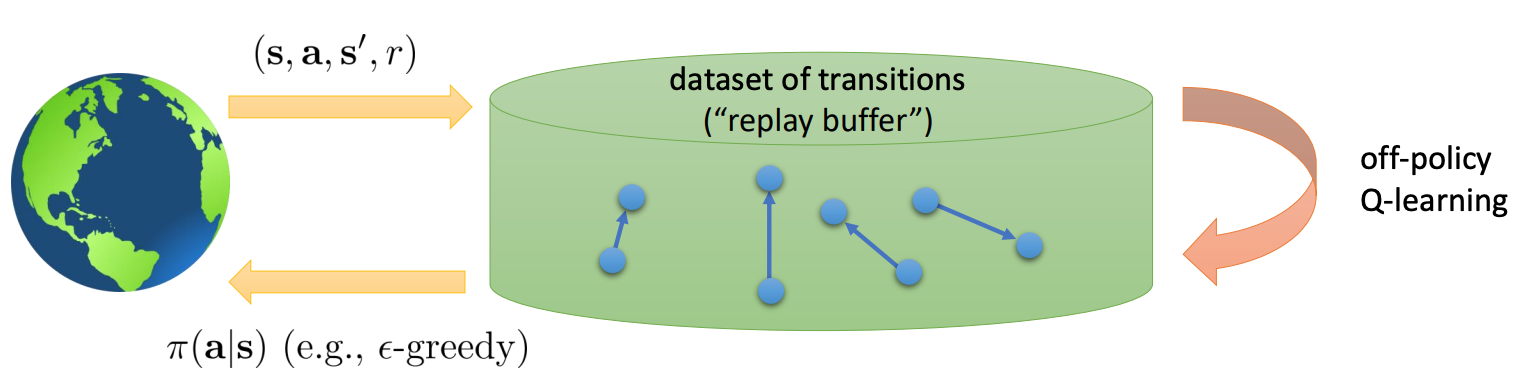
\includegraphics[scale=0.5]{figures/qwrb.png}
    \caption{Q-learning with replay buffers}
    \label{fig:qwfb}
\end{figure}


Putting it all together, we sketch out the full Q-learning algorithm with replay buffer in Alg. \ref{alg:QwRB}.
\begin{algorithm}[t!]
\caption{Q-Learning with Replay Buffer}
\begin{algorithmic}[1]
\label{alg:QwRB}
\REQUIRE Some base policy for data collection; hyperparameter $K$
\WHILE{true}
    \STATE Collect dataset $\{(s_i,a_i,s'_i,r_i)\}$ using some policy, add it to replay buffer $\mathcal{B}$
    \FOR{$K$ times}
        \STATE Sample a batch $(s_i,a_i,s'_i,r_i)$ from $\mathcal{B}$
        \STATE Set $y_i\leftarrow r(s_i,a_i) + \gamma \max_{a'_i}Q_\phi(s'_i,a'_i)$
        \STATE Set $\phi \leftarrow \phi-\alpha\Sigma_i\frac{dQ_\phi}{d\phi}(s_i,a_i)(Q_\phi(s_i,a_i) - y_i)$
    \ENDFOR
\ENDWHILE
\end{algorithmic}
\end{algorithm}
What have changed here in Alg. \ref{alg:QwRB} compared with Alg. \ref{alg:fittedQ}? In step 2, we are not only collecting dataset, but also adding the dataset to replay buffer $\mathcal{B}$. Inside the for loop, we are now sampling a batch of transitions from $\mathcal{B}$, which will bring us lower variance when we take the gradient step on the batch. We also periodically update $\mathcal{B}$.

The above solution solves the correlation problem, but we still need to address the wrong gradient problem. 

\section{Target Networks}
To solve the wrong gradient problem, we are essentially trying to solve the problem that the target value $y_i$ is heavily dependent on our gradient parameter $\phi$. Therefore, one way to improve this is to use a separate Q-function with another parameter $\phi'$ in order to decorrelate the two values. We should also use a well-defined $\phi'$, which can be set as the $\phi$ parameter 1000 steps ago. When setting $y_i$, we set it from the Q function with another parameter, thus decorrelating the two values. Together with the use of replay buffer, we alleviated the wrong policy and the correlation samples problems, as shown in Alg. \ref{alg:QwRB_tn}.
\begin{algorithm}[t!]
\caption{Q-Learning with Replay Buffer and Target Network}
\begin{algorithmic}[1]
\label{alg:QwRB_tn}
\REQUIRE Some base policy for data collection; hyperparameter $K$ and $N$
\WHILE{true}
\STATE Save target network parameters: $\phi' \leftarrow \phi$
\FOR{$N$ times}
    \STATE Collect dataset $\{(s_i,a_i,s'_i,r_i)\}$ using some policy, add it to replay buffer $\mathcal{B}$
    \FOR{$K$ times}
        \STATE Sample a batch $(s_i,a_i,s'_i,r_i)$ from $\mathcal{B}$
        \STATE Set $y_i\leftarrow r(s_i,a_i) + \gamma \max_{a'_i}Q_{\phi'}(s'_i,a'_i)$
        \STATE Set $\phi \leftarrow \phi-\alpha\Sigma_i\frac{dQ_\phi}{d\phi}(s_i,a_i)(Q_\phi(s_i,a_i) - y_i)$
    \ENDFOR
    \ENDFOR
\ENDWHILE
\end{algorithmic}
\end{algorithm}
Here we are frequently sampling batches from $\mathcal{B}$ and taking the gradient steps. We are less frequently updating the replay buffer as discussed in Alg. \ref{alg:QwRB}. We are even less frequently updating the network parameters, since we said one good choice for parameter $\phi'$ is to use $\phi$ 1000 steps ago.

Using target networks and replay buffers, we can sketch out a classic deep Q-learning algorithm (DQN), proposed by Minh et al. in \cite{mnih2013playing}. The pseudocode is in \ref{alg:dqn}. Here we choose $N$ to be a large number because our intention is to infrequently update the parameters. To further optimize the algorithm, it might feel weird abruptly update $\phi'$ after $N$ steps. Therefore, to alleviate this ``abruptness'', we can use \textbf{Polyak Averaging}: in step 6 of Alg. \ref{alg:dqn}, instead of copying $\phi$ every $N$ steps, we do $\phi' \leftarrow \tau\phi' + (1-\tau)\phi$. We also call such update a damped update.
\begin{algorithm}[t!]
\caption{Classic Deep Q-Learning Algorithm (DQN)}
\begin{algorithmic}[1]
\label{alg:dqn}
\WHILE{true}
    \STATE Take some action $a_i$ and observe $(s_i,a_i,s'_i,r_i)$ and add it to $\mathcal{B}$
    \STATE Sample mini-batch $\{s_j,a_j,s'_j,r_j\}$
    \STATE Compute $y_j = r_j + \gamma \max_{a'_j}Q_{\phi'}(s'_j,a'_j)$ using target network $Q_{\phi'}$
    \STATE $\phi \leftarrow \phi-\alpha\Sigma_j\frac{dQ_\phi}{d\phi}(s_j,a_j)(Q_\phi(s_j,a_j) - y_J)$
    \STATE update $\phi'$: copy $\phi$ every $N$ steps.
\ENDWHILE
\end{algorithmic}
\end{algorithm}

Now let us view the three different Q-learning algorithms in a more general way. As shown in Fig. \ref{fig:dqn}, there are three different steps in the algorithm. The first step is to collect data, the second step is to update the target in the target network, and the third step is to regress onto the Q-function. In the simplest, regression-based fitted Q-learning algorithm, process 3 is in the inner loop of process 2, which is in the inner loop of process 1. In online Q-learning, we evict the old transitions immediately, and process 1, 2, and 3 run at the same speed. In DQN, process 1 and 3 run at the same speed, but process 2 runs slower.
\begin{figure}
    \centering
    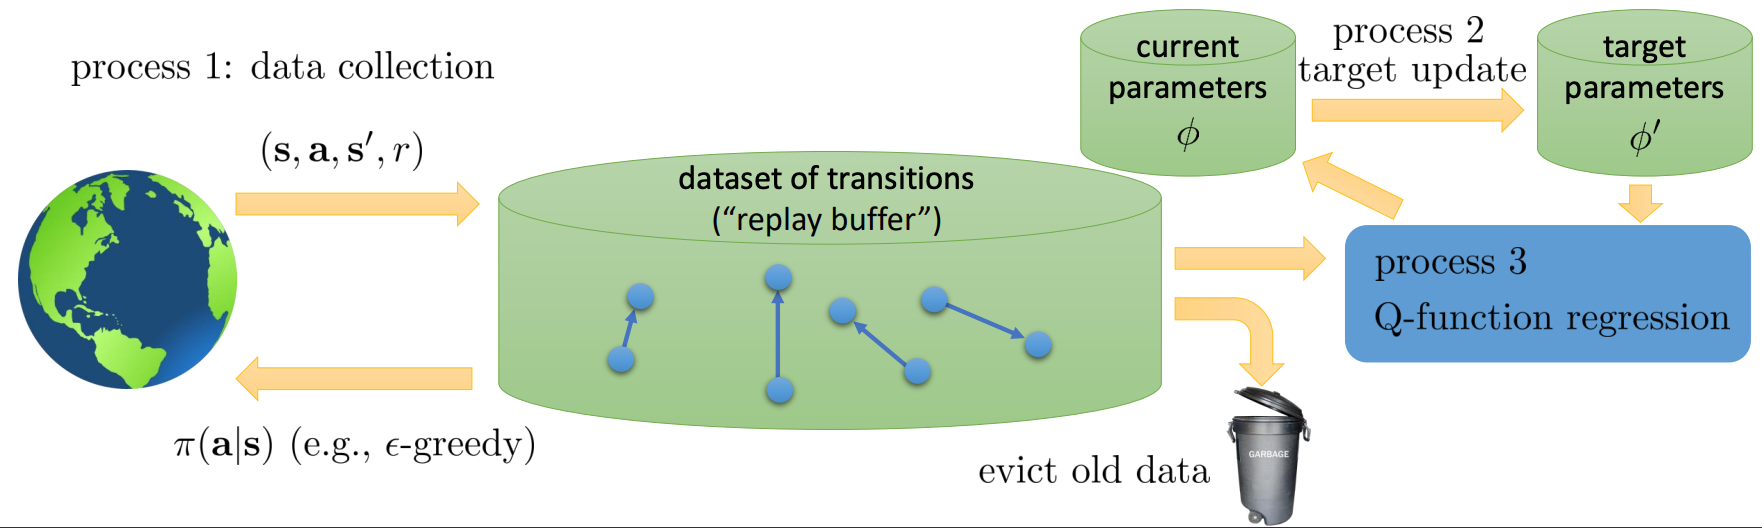
\includegraphics[scale=0.5]{figures/dqn.png}
    \caption{Q-learning in a more general view.}
    \label{fig:dqn}
\end{figure}

\section{Inaccuracy in Q-Learning}
Q-values are not necessarily accurate. The reason lies in the target value. Recall that the target value $y$ is defined as $y_j = r_j + \gamma \max_{a'_j}Q_{\phi'}(s'_j,a'_j)$. The $\max$ operation in the target is the main problem, because for two random variables $X_1$ and $X_2$, $\mathbb{E}[\max(X_1,X_2)] \geq \max(\mathbb{E}[X_1],\mathbb{E}[X_2])$. Therefore, when $Q_{\phi'}(s'_j,a'_j)$ is noisy, the max operation is going to overestimate the next Q-value.

\subsection{Double Q-Learning}
One might notice that $\max_{a'}Q_{\phi'}(s',a') = Q_{\phi'}(s',\argmaxA_{a'}Q_{\phi'}(s',a'))$. Thus, if we somehow managed to decorrelate the error from the selected action and the error from the Q-function, we could eliminate the erroneous overestimation. To achieve this, we can use two different networks to choose actions and evaluate the Q-function values. 
\begin{align*}
    Q_{\phi_A}(s,a) &\leftarrow r + \gamma Q_{\phi_B}\left(s',\argmaxA_{a'}Q_{\phi_A}(s',a')\right)\\
    Q_{\phi_B}(s,a) &\leftarrow r + \gamma Q_{\phi_A}\left(s',\argmaxA_{a'}Q_{\phi_B}(s',a')\right)
\end{align*}
Essentially we are using one network's parameter to update the value, while using the other's to select the action. Using the two separate networks, we are decorrelating the action selection and value evaluation errors, thus decreasing the overestimation in the Q-values.

In practice, we can just use the actual and target networks for the two separate networks. Therefore, instead of setting target $y$ as $y = r + \gamma Q_{\phi'}\left(s',\argmaxA_{a'}Q_{\phi'}(s',a')\right)$, we use the current network to select action, and use the target network to evaluate value: $y = r + \gamma Q_{\phi'}\left(s',\argmaxA_{a'}Q_{\phi}(s',a')\right)$.

\subsection{N-Step Return Estimator}
In the definition of our target $y$, $y_{i,t} = r_{i,t} + \max_{a_{i,t+1}}Q_{\phi'}(s_{i,t+1},a_{i,t+1})$, the Q-value only matters if it is a good estimate. If the Q-value estimate is bad, the only values that matter are from the reward term, so we are not learning much about the Q-function. To resolve this problem, let us recall the N-step cut trick we did in the actor-critic algorithm. In actor-critic algorithm, to leverage the bias and variance tradeoff in policy gradient, we can end the trajectory earlier, and only count the reward summed up to $N$ steps from now. Specifically, we can define the target as:
$$y_{i,t} = \sum_{t'=t}^{t+N-1}\gamma^{t-t'}r_{i,t} +\gamma^N \max_{a_{i,t+1}}Q_{\phi'}(s_{i,t+1},a_{i,t+1})$$
One subtle problem with this solution is that the learning process suddenly becomes on-policy, so we cannot efficiently make use of the off-policy data. Why is it on-policy? If we look at the summation of the rewards, we are collecting the rewards data using a certain trajectory, which is generated by a specific policy. Therefore, we end up having less biased target values when the Q-values are inaccurate, and in practice, it is faster in early stages of learning. However, it is only correct when we are learning on-policy. To fix this problem, one could ignore this mismatch, which somehow works very well in practice. Or one could cut the trace by dynamically adapting $N$ to get only on-policy data. Also, one could use importance sampling as we discussed before. For more details, please refer to this paper by Munos et al. \cite{munos2016safe}.
\subsection{Q-Learning with Continuous Actions}
Recall the implicit policy that we define using Q-learning:
\begin{align*}
\pi'(a_t|s_t) & = \begin{cases}
                1, & \mathrm{if } \;a_t = \argmaxA_{a_t}A^\pi(s_t,a_t)\\
                 0, & \mathrm{otherwise}
                    \end{cases}
\end{align*}
One problem with this definition is that the $\argmaxA$ operation cannot be easily applied if the actions are continuous. How are we going to address such an issue?

One option is to use various optimization techniques, as one may have seen in UC Berkeley's EE 127. Specifically, one could use SGD on the action space to produce an optimal $a_t$ by solving an optimization problem. Another simple approach is to stochastically optimize the Q-values by using some samples of the values from some pre-defined distribution (e.g. uniform): $\max_a Q(s,a) \simeq \max \{Q(s,a_1), ..., Q(s,a_N)\}$. One could also improve the accuracy by using some more sophisticated optimization techniques such as Cross-Entropy Method (CEM).

Option no. 2 is to use function classes that are easy to maximize. For example, one could use the Normalized Advantage Functions (NAF) proposed by Gu et al. in \cite{gu2016continuous}.

Another rather fancier option is to learn an approximate optimizer, which was originally proposed by Lillicrap et al. in \cite{lillicrap2015continuous}. The idea of Deep Deterministic Policy Gradient (which is actually a Q-learning in disguise) is to train another network $\mu_\theta(s)$ such that $\mu_\theta(s) \simeq \argmaxA_a Q_\phi(s,a)$. To train the network, one can see that the optimization of Q-function with respect to $\theta$ can be solved by $\theta \leftarrow \argmaxA_\theta Q_\phi(s,\mu_\theta(s))$ because by chain rule, $\frac{dQ_\phi}{d\theta} = \frac{da}{d\theta}\frac{dQ_\theta}{da}$. Then the new target becomes:
$$y_j = r_j + \muQ_{\phi'}(s'_j,\mu_\theta(s'_j))\simeq r_j + \muQ_{\phi'}(s'_j, \argmaxA_{a'}Q_{\phi'}(s'_j,a'_j))$$

The sketch of DDPG is in Alg. \ref{alg:ddpg}. In step 5, we are updating the Q-function, and in step 6, we are updating the argmax-er. Therefore, DDPG is essentially DQN with argmax-er.
\begin{algorithm}[t!]
\caption{Deep Deterministic Policy Gradient (DDPG)}
\begin{algorithmic}[1]
\label{alg:ddpg}
\WHILE{true}
    \STATE Take some action $a_i$ and observe $(s_i,a_i,s'_i,r_i)$ and add it to $\mathcal{B}$
    \STATE Sample mini-batch $\{s_j,a_j,s'_j,r_j\}$
    \STATE Compute $y_j = r_j + \gamma \max_{a'_j}Q_{\phi'}(s'_j,a'_j)$ using target networks $Q_{\phi'}$ and $\mu_{\theta'}$
    \STATE $\phi \leftarrow \phi-\alpha\Sigma_j\frac{dQ_\phi}{d\phi}(s_j,a_j)(Q_\phi(s_j,a_j) - y_J)$
    \STATE $\theta \leftarrow \theta + \beta\sum_j\frac{da}{d\theta}(s_j)\frac{dQ_\phi}{da}(s_j,a)$
    \STATE update $\phi'$ and $\theta'$
\ENDWHILE
\end{algorithmic}
\end{algorithm}


